% --- ORIENTADOR (0.1%): ---
% Este é o Capítulo 1 revisado.
% Eu reescrevi a Justificativa, Objetivos e Estrutura para
% responder DIRETAMENTE ao feedback da sua banca.
% --- FIM DO COMENTÁRIO ---

% --- ORIENTADOR (0.1%): ---
% Este é o Capítulo 1 revisado.
% Eu reescrevi a Justificativa, Objetivos e Estrutura para
% responder DIRETAMENTE ao feedback da sua banca.
% --- FIM DO COMENTÁRIO ---

\chapter{Introdução}

\section{Introdução}
% --- ORIENTADOR: Esta seção está boa, mantemos o texto original.
A presença de animais de estimação nos lares tornou-se um fenômeno social de grande relevância.
Essa transformação na dinâmica familiar, no entanto, colide com os desafios da vida moderna, onde rotinas de trabalho e compromissos diários frequentemente resultam em longos períodos de ausência dos tutores, comprometendo a regularidade e a qualidade dos cuidados essenciais \cite{rodrigues2019}.
Falhas no manejo da dieta podem levar a problemas de saúde como obesidade ou desnutrição \cite{alves2020}, enquanto a falta de água fresca e um ambiente termicamente inadequado são fatores diretos que podem causar desidratação e estresse fisiológico, comprometendo a capacidade de termorregulação do animal.


Nesse contexto, a tecnologia, em particular a Internet das Coisas (IoT), surge como uma poderosa aliada.
O mercado global de cuidados tecnológicos para animais de estimação (pets) reflete essa tendência, com o segmento de alimentadores inteligentes estimado em USD 1,46 bilhão em 2024 e com projeção de crescimento para USD 2,35 bilhões até 2030 \cite{grandview2024}.
Essa demanda é impulsionada pela busca por conveniência e pela crescente conscientização sobre o bem-estar animal.
Contudo, apesar da proliferação de dispositivos, o mercado ainda é dominado por soluções que operam de forma isolada, tratando o cuidado animal de maneira fragmentada.
O conceito de ``bem-estar animal'' pode ser tecnicamente aprofundado pela literatura da Pecuária de Precisão (\textit{Precision Livestock Farming} - PLF), que utiliza sensores para monitorar o microclima (temperatura, umidade, gases) e seu impacto direto na saúde e produtividade dos animais \cite{tavares2021, neethirajan2017}.
Isso demonstra que o monitoramento ambiental não é apenas uma funcionalidade adicional, mas um pilar para a saúde animal \cite{mdpiAnimals2024}.
Este trabalho, originado a partir de um projeto desenvolvido na disciplina de Sistemas Integrados de Hardware e Software I, propõe-se a documentar e validar um sistema inteligente de monitoramento e automação para ambientes de animais domésticos, com um foco crítico na arquitetura e na seleção de componentes.
\section{Justificativa}

% --- ORIENTADOR: INÍCIO DA EDIÇÃO (FEEDBACK DA BANCA) ---
% O texto abaixo foi reescrito para abordar o feedback:
% 1. 'Justificativa não tem um ambiente conjugado'
% 2. 'Solução de baixo custo… como reforço'
% 3. 'Verificar se existe outros iguais no mercado'
% 4. 'Aplicar mais a Engenharia software'
% --- FIM DO COMENTÁRIO ---

A justificativa para este projeto reside em uma lacuna crítica não endereçada pela maioria das soluções comerciais de cuidado animal: a fragmentação funcional.
Uma análise do mercado (como em \cite{jacomini2024, circat_paper}) revela um arquipélago de dispositivos proprietários e isolados: alimentadores que não se comunicam com bebedouros, e sistemas de monitoramento ambiental que não influenciam a lógica de automação.
Essa abordagem em silos impede uma visão holística e proativa do bem-estar do animal, tratando sintomas (ex: um pote de ração vazio) em vez de gerenciar um \textbf{ecossistema de cuidado conjugado}.
Adicionalmente, as soluções comerciais existentes são frequentemente ``caixas-pretas'' de custo elevado, que limitam a personalização e a integração.
Este projeto justifica-se, portanto, pelo uso de uma \textbf{abordagem de baixo custo} como um facilitador estratégico.
A utilização de tecnologias abertas como o microcontrolador ESP32, o protocolo Message Queuing Telemetry Transport (MQTT) e a plataforma de fluxo Node-RED não apenas viabiliza uma solução financeiramente acessível, mas, fundamentalmente, fornece a \textbf{flexibilidade arquitetural} necessária para criar uma plataforma de orquestração centralizada e unificada.
Em resposta direta a essa lacuna, este projeto propõe a concepção e validação de um sistema que atua como essa plataforma de orquestração.
Indo além da simples automação, a solução sugerida integra e correlaciona múltiplos fatores críticos: a quantidade de ração disponível, o nível de água e as condições de temperatura e umidade, tratando-os não como problemas isolados, mas como um \textbf{ambiente conjugado} e interdependente.
Do ponto de vista acadêmico, o trabalho representa a aplicação prática de conhecimentos de diversas áreas de Sistemas de Informação.
Como resposta direta ao \textit{feedback} da banca avaliadora do Trabalho de Conclusão de Curso (TCC) 1, o TCC 2 aprofunda a \textbf{aplicação de princípios da Engenharia de Software}, focando na validação de uma arquitetura de nuvem escalável e na implementação de um módulo de análise de dados para validação do sistema em um ambiente controlado.
Socialmente, o projeto sugere um caminho para impactar positivamente a relação entre tutores e seus animais, reduzindo o estresse relacionado à ausência e contribuindo para a promoção da saúde e do bem-estar animal.
% --- ORIENTADOR: FIM DA SEÇÃO EDITADA ---

\section{Objetivos}
O desenvolvimento deste trabalho é norteado pelos seguintes objetivos:

\subsection{Objetivo Geral}
Desenvolver e validar um sistema embarcado para o monitoramento e a automação do controle de temperatura, alimentação e hidratação de animais domésticos, com notificações em tempo real, painel de controle interativo e integração com serviços de nuvem para controle por voz e análise preditiva.
% --- ORIENTADOR: INÍCIO DA EDIÇÃO (FEEDBACK DA BANCA + NOVAS FEATURES) ---
% Adicionando os objetivos do TCC 2 (Features 1 e 2)
% e um objetivo específico sobre Engenharia de Software,
% como a banca pediu ('Aplicar mais a Engenharia software').
% --- FIM DO COMENTÁRIO ---
\subsection{Objetivos Específicos}
\begin{itemize}
    \item Implementar sensores para a medição contínua dos níveis de água e ração nos recipientes e reservatórios, bem como da temperatura e umidade do ambiente;
\item Integrar os sensores a um microcontrolador ESP32, programando-o para coletar e transmitir os dados via protocolo MQTT;
\item Desenvolver um sistema de notificações em tempo real via Telegram para alertar o tutor sobre eventos críticos;
\item Estruturar um banco de dados relacional (MySQL) para o armazenamento de dados históricos;
\item Criar um painel de controle (dashboard) em Node-RED para a visualização dos dados em tempo real e o controle manual dos atuadores;
\item Validar a funcionalidade e a precisão do protótipo por meio de testes em um ambiente simulado (Wokwi);
% --- NOVOS OBJETIVOS TCC 2 ---
    \item \textbf{(TCC 2)} Aplicar princípios de Engenharia de Software para evoluir a arquitetura do protótipo para uma solução de nuvem segura, profissional e escalável, utilizando serviços da Amazon Web Services (AWS IoT Core e Lambda);
\item \textbf{(TCC 2)} Desenvolver e validar a integração com assistentes de voz (Amazon Alexa), permitindo o controle de múltiplos atuadores do sistema por comandos de voz;
\item \textbf{(TCC 2)} Implementar e validar um módulo de saúde preditiva em um \textbf{ambiente controlado}, aplicando técnicas de \textit{Machine Learning} (ML) (Isolation Forest) para detectar anomalias nos padrões de consumo de dados históricos, como um indicador precoce de problemas de saúde animal;
\end{itemize}
% --- ORIENTADOR: FIM DA SEÇÃO EDITADA ---

\section{Estrutura do Trabalho}
% --- ORIENTADOR: INÍCIO DA EDIÇÃO (NOVO ESCOPO TCC 2) ---
% Esta nova estrutura descreve o TCC 2 finalizado.
% Ela substitui a estrutura antiga do TCC 1.
% --- FIM DO COMENTÁRIO ---
Este trabalho está organizado da seguinte forma: o \textbf{Capítulo 2} apresenta a fundamentação teórica, revisando os principais conceitos de IoT e as novas tecnologias de nuvem e \textit{Machine Learning} empregadas.
O \textbf{Capítulo 3} detalha a metodologia de Prototipagem Evolucionária e a abordagem de validação em ambiente controlado.
O \textbf{Capítulo 4} descreve a arquitetura do sistema, desde a concepção do protótipo simulado (TCC 1) até a arquitetura de nuvem final (TCC 2), que segue os princípios de Engenharia de Software.
O \textbf{Capítulo 5} apresenta a implementação e os resultados do Módulo de Saúde Preditiva (Feature 1).
O \textbf{Capítulo 6} detalha a implementação e os testes de validação da integração com a nuvem AWS e a assistente de voz Alexa (Feature 2).
Finalmente, o \textbf{Capítulo 7} apresenta as conclusões finais do trabalho e sugere os próximos passos para a evolução do projeto.












\chapter{Fundamentação Teórica}
Este capítulo aborda os conceitos e tecnologias essenciais que fundamentam o desenvolvimento do projeto.
\section{Internet das Coisas (IoT) no Cuidado Animal}
A Internet das Coisas (IoT) refere-se à interconexão de dispositivos físicos que coletam e compartilham dados pela internet.
No setor de cuidados com animais, a IoT possibilita a criação de ecossistemas inteligentes que melhoram a qualidade de vida dos animais de estimação (pets) e oferecem conveniência aos tutores \cite{rodrigues2019, iotah_review2020}.
Soluções como coleiras com GPS, câmeras interativas e, de especial interesse para este trabalho, comedouros e bebedouros inteligentes, são exemplos práticos dessa aplicação.
Esses sistemas não apenas automatizam tarefas, mas também permitem um cuidado proativo, baseado em dados, ao monitorar a saúde e o comportamento do animal, alinhando-se aos princípios da Pecuária de Precisão (PLF), onde o monitoramento contínuo de parâmetros de saúde e ambiente é fundamental para o bem-estar \cite{jacomini2024, plf_overview2022, ilvo_plf}.
\section{Sistemas Embarcados e o Microcontrolador ESP32}
Sistemas embarcados são sistemas computacionais dedicados a funções específicas dentro de um sistema maior \cite{jacomini2024}.
O coração desses sistemas é, frequentemente, um microcontrolador. Para este projeto, foi escolhido o \textbf{ESP32}, um microcontrolador de baixo custo da Espressif Systems.
A escolha se justifica por suas características robustas, que incluem um processador dual-core, conectividade Wi-Fi e Bluetooth integradas, e um vasto conjunto de periféricos de entrada/saída (como General Purpose Input/Output (GPIOs), ADC, Pulse Width Modulation (PWM)), tornando-o ideal para aplicações de IoT que exigem processamento, conectividade e controle de múltiplos sensores e atuadores \cite{jacomini2024}.
% --- ORIENTADOR: INÍCIO DA EDIÇÃO (FEEDBACK DA BANCA) ---
% Trocando ``Análise Crítica'' por ``Levantamento'', como solicitado.
\section{Levantamento de Componentes: Sensores e Atuadores}
A confiabilidade de um sistema de cuidado animal depende diretamente da precisão e robustez de seus componentes.
A seguir, é apresentado um \textbf{levantamento} das escolhas de hardware.
% --- FIM DA EDIÇÃO ---

\subsection{Sensor de Peso (Célula de Carga e Módulo HX711)}
Para medir a quantidade de ração, a combinação de uma célula de carga com o módulo HX711 é uma escolha interessante.
O HX711 é um conversor analógico-digital (ADC) de 24 bits de alta resolução, projetado especificamente para amplificar e converter os minúsculos sinais elétricos de pontes de Wheatstone (como as encontradas em células de carga), tornando-o ideal para medições de peso precisas e de baixo custo \cite{hx711_guide, hx711_tech}.
A obtenção de leituras estáveis, no entanto, exige um processo cuidadoso de calibração e a implementação de algoritmos de filtragem de software para mitigar ruídos, um desafio prático abordado na Seção.
% --- ORIENTADOR: INÍCIO DA EDIÇÃO (FEEDBACK DA BANCA) ---
% 'Suavizando' o título e a linguagem.
\subsection{Sensor de Nível de Água: Levantamento de Alternativas}
\label{sec:sensor_agua}

A escolha inicial de um sensor ultrassônico de baixo custo como o HC-SR04 para medir o nível de água serviu como uma prova de conceito inicial.
Contudo, um levantamento da literatura e dos requisitos de confiabilidade do sistema sugere que esta pode ser uma escolha adequada para um protótipo estruturado.
A precisão de sensores ultrassônicos é notoriamente afetada por fatores como espuma, turbulência na superfície, umidade e variações de temperatura, que alteram a velocidade do som \cite{ultrasonic_foam, ultrasonic_limitations, ultrasonic_temp_humidity}.
% --- FIM DA EDIÇÃO ---

Para endereçar proativamente essa vulnerabilidade, foi realizada uma análise comparativa abrangente, contrastando tecnologias de medição sem contato (ultrassom, laser) com uma abordagem de medição de contato e discreta (sensor de boia).
Essa análise, consolidada na Tabela~\ref{tab:water_sensor_comparison}, avalia não apenas o custo, mas o princípio de funcionamento, a natureza da medição (contínua vs. discreta) e a resiliência de cada tecnologia frente aos desafios de um bebedouro para animais.
\begin{table}[H]
\centering
\caption{Análise Comparativa de Tecnologias para Medição de Nível de Água.}
\label{tab:water_sensor_comparison}
\resizebox{\textwidth}{!}{%
\begin{tabular}{|l|p{3.5cm}|p{3.5cm}|p{3.5cm}|p{3.5cm}|}
\hline
\textbf{Característica} & \textbf{HC-SR04 (Ultrassônico)} & \textbf{VL53L1X (ToF - Laser)} & \textbf{Sensor de Boia (Mecânico)} \\ \hline
\textbf{Princípio} & Tempo de Voo (Som) & Tempo de Voo (Luz IR) & Chave magnética (Reed Switch) acionada por flutuador.
\\ \hline
\textbf{Tipo de Medição} & Contínua (analógica) & Contínua (analógica) & Discreta (digital: cheio/vazio) \\ \hline
\textbf{Contato com Água} & Não & Não & Sim (imerso) \\ \hline
\textbf{Prós} & Custo irrisório, simplicidade de prova de conceito.
Fornece medição contínua do nível. & Altíssima precisão (mm), imune a espuma/vapor, feixe estreito ideal para recipientes pequenos.
& Altíssima confiabilidade para detecção de ponto único, baixo custo, imune a todas as condições da água (espuma, turbidez, vapor).
Simplicidade elétrica. \\ \hline
\textbf{Contras} & Não é à prova d'água, muito sensível a espuma, vapor e turbulência \cite{ultrasonic_foam}.
Precisão afetada pela temperatura \cite{ultrasonic_temp_humidity}. & Pode ler o fundo do recipiente com água clara, requerendo calibração.
Sensível à luz solar direta. Custo mais elevado. & Fornece apenas uma medição binária (um ponto de nível), não o volume exato.
Risco de contaminação e desgaste mecânico por ter partes móveis imersas. \\ \hline
\textbf{Adequação} & Prova de conceito.
Inadequado para um produto final confiável. & Excelente para monitoramento preciso e contínuo, mas exige ambiente controlado e possível calibração de software.
& Ideal como sistema de segurança (ex: detectar nível mínimo para acionar alerta/enchimento) ou para lógica simples, mas insuficiente para monitoramento detalhado do consumo.
\\ \hline
\end{tabular}%
}
\caption*{Fonte: Elaborado pelo autor (2025).}
\end{table}

Esta análise informa que a escolha da tecnologia de sensoriamento de água é um \textit{trade-off} fundamental entre a granularidade da informação e a robustez da medição.
Enquanto sensores ToF oferecem dados ricos e contínuos, sua complexidade e sensibilidade são maiores.
Em contrapartida, um sensor de boia oferece uma informação binária, porém extremamente confiável.
Para os fins deste projeto, que visa um monitoramento detalhado, a abordagem sem contato permanece preferencial, mas a vulnerabilidade do HC-SR04 aponta para a necessidade de sua substituição por uma tecnologia mais resiliente, como o ToF, ou a hibridização com um sensor de boia para redundância de segurança em trabalhos futuros.
\subsection{Sensor de Temperatura e Umidade (DHT11 vs. DHT22)}
Para o monitoramento ambiental, a escolha entre os sensores da família DHT deve ser bem fundamentada.
O DHT22, embora ligeiramente mais caro, é tecnicamente superior ao DHT11, oferecendo maior precisão e uma faixa de operação mais ampla, fatores cruciais para garantir o conforto térmico do animal.
A Tabela~\ref{tab:dht_comparison} detalha as diferenças.

\begin{table}[H]
\centering
\caption{Comparativo técnico entre os sensores DHT11 e DHT22.
Fonte: Compilado de \cite{dht_compare_seeed, dht_compare_randomnerd, dht_compare_pcbasic}.}
\label{tab:dht_comparison}
\begin{tabular}{|l|l|l|}
\hline
\textbf{Característica} & \textbf{DHT11} & \textbf{DHT22 (AM2302)} \\ \hline
Faixa de Temperatura & $0^{\circ}$C a $50^{\circ}$C & $-40^{\circ}$C a $80^{\circ}$C \\ \hline
Precisão da Temperatura & $\pm2^{\circ}$C & $\pm0.5^{\circ}$C \\ \hline
Faixa de Umidade & 20\% a 90\% RH & 0\% a 100\% RH \\ \hline
Precisão da Umidade & $\pm5\%$ RH & $\pm2\%$ RH \\ \hline
\end{tabular}
\end{table}

\subsection{Atuadores (Servo Motor e Válvula Solenoide)}

A automação das tarefas de alimentação e hidratação depende de atuadores confiáveis para o controle físico dos insumos.

Para o controle de porções de ração, foi selecionado um \textbf{Servo Motor}. A justificativa para esta escolha, validada em trabalhos como o de \cite{alves2020}, reside na sua capacidade de \textbf{controle de precisão angular}. Diferente de um motor DC comum (que apenas gira continuamente), um servo motor pode ser instruído a girar para um ângulo exato (ex: 90 graus) e retornar. Essa característica é ideal para implementar um dispensador do tipo rosca ou alavanca, onde o ângulo de rotação é diretamente proporcional ao volume de ração dispensado, garantindo a consistência das porções.

Para o controle do fluxo de água, a escolha foi uma \textbf{Válvula Solenoide}. Este componente atua como um portão eletromagnético (on/off) para líquidos. Sua principal vantagem é a \textbf{simplicidade e robustez} para o controle binário (liberar ou bloquear a água), sendo facilmente controlada por um microcontrolador (através de um relé ou transistor), o que a torna uma escolha direta e eficaz para a automação do reabastecimento do bebedouro.



\section{Protocolo de Comunicação MQTT e Qualidade de Serviço (QoS)}

O \textbf{Message Queuing Telemetry Transport (MQTT)} é um protocolo de mensagens leve, baseado no padrão publicar/assinar, ideal para ambientes de IoT com recursos limitados \cite{rodrigues2019, mqtt_aws}.
Sua arquitetura desacopla os dispositivos, tornando o sistema modular e escalável.
Para aplicações críticas, é essencial compreender os níveis de \textbf{Qualidade de Serviço (QoS)} \cite{mqtt_qos_bevywise}:
\begin{itemize}
    \item \textbf{QoS 0 (At most once):} ``Dispare e esqueça''.
Entrega rápida, mas sem garantia. Adequado para dados não críticos, como leituras de temperatura periódicas, onde a perda ocasional de um pacote é aceitável \cite{mqtt_qos_cedalo}.
\item \textbf{QoS 1 (At least once):} Garante que a mensagem seja entregue pelo menos uma vez, com confirmação.
Pode haver duplicatas. É o padrão de fato para comandos em plataformas de nuvem gerenciadas.
\item \textbf{QoS 2 (Exactly once):} Garante que a mensagem seja entregue exatamente uma vez, através de um \textit{handshake} de quatro etapas.
É o nível *teórico* mais confiável, porém mais lento \cite{mqtt_qos_bevywise, mqtt_qos_thingsboard}.
\end{itemize}

É crucial notar que, embora o QoS 2 seja o ideal teórico para comandos críticos (como ``alimentar o pet''), as principais plataformas de nuvem, incluindo o \textbf{AWS IoT Core}, não implementam o QoS 2, limitando o suporte ao QoS 0 e QoS 1.
Conforme a própria documentação da AWS, ``AWS IoT doesn't support publishing or subscribing with QoS level 2'' \cite{aws_iot_core_docs}.
Esta é uma decisão de engenharia da plataforma: a complexidade e a latência do QoS 2 são trocadas pela simplicidade e velocidade do QoS 1. A responsabilidade de garantir a entrega ``exatamente uma vez'' (prevenção de duplicatas) é, portanto, movida da camada de protocolo (MQTT) para a \textbf{camada de aplicação} (a lógica do \textit{software}, como a implementação de idempotência no \textit{handler} do AWS Lambda) \cite{aws_lambda_docs, aws_alexa_iot}.
Adicionalmente, a segurança do MQTT não é nativa; ele depende de camadas de transporte seguras como o TLS para criptografar os dados em trânsito \cite{mqtt_security_review, mqtt_aws}.
\begin{table}[H]
\centering
\caption{Aplicação Estratégica dos Níveis de Qualidade de Serviço (QoS) do MQTT no contexto do TCC}
\label{tab:qos_application}
\resizebox{\textwidth}{!}{%
\begin{tabular}{|p{2.8cm}|p{6.6cm}|p{2cm}|p{1.5cm}|p{7.5cm}|}
\hline
\textbf{Tipo de Mensagem} & \textbf{Tópico Exemplo} & \textbf{Criticidade} & \textbf{QoS Escolhido} & \textbf{Justificativa Técnica} \\ \hline
Dados de Sensor (Temperatura/Umidade) & \texttt{canil/ambiente/temperatura} & Baixa & QoS 0 & A perda ocasional de uma leitura ambiental não compromete o sistema.
Prioriza-se a baixa latência e o mínimo de sobrecarga \cite{mqtt_qos_cedalo}.
\\ \hline
Dados de Sensor (Nível de Ração/Água) & \texttt{canil/racao/tigela/peso} & Média & QoS 1 & Garante que a mensagem seja entregue \textbf{pelo menos uma vez}.
É importante que o dashboard e a lógica de alerta recebam os dados.
\\ \hline
Comando do Atuador (Liberar Água) & \texttt{canil/agua/valvula/comando} & Média & QoS 1 & Garante a entrega do comando.
Uma execução duplicada não é catastrófica, tornando o QoS 1 um bom equilíbrio entre confiabilidade e complexidade \cite{mqtt_qos_bevywise}.
\\ \hline
Comando do Atuador (Dispensar Ração) & \texttt{canil/racao/servo/comando} & Alta & \textbf{QoS 1} \textit{(Forçado pela Nuvem)} & Embora o QoS 2 seja o ideal teórico para evitar duplicatas \cite{mqtt_qos_bevywise}, a plataforma de nuvem escolhida (AWS IoT Core) não o suporta.
A garantia de ``pelo menos uma vez'' (QoS 1) é aceita, e a lógica de prevenção de duplicatas (idempotência) é movida para a camada de aplicação (AWS Lambda) \cite{aws_lambda_docs, aws_alexa_iot}.
\\ \hline
\end{tabular}%
}
\end{table}

% --- ORIENTADOR: O RESTANTE DA SEÇÃO (sobre o 'overhead' do QoS) FOI MANTIDO ---
É crucial notar que a aplicação estratégica dos níveis de QoS, detalhada na Tabela~\ref{tab:qos_application}, implica um \textit{trade-off} direto de desempenho e consumo de recursos.
A confiabilidade não é isenta de custos: o QoS 0 representa a linha de base com uma única mensagem \texttt{PUBLISH}.
O QoS 1 dobra o tráfego de rede para aquela mensagem, exigindo uma confirmação (\texttt{PUBACK}).
Já o QoS 2, o mais robusto, quadruplica o fluxo com um \textit{handshake} de quatro etapas (\texttt{PUBLISH}, \texttt{PUBREC}, \texttt{PUBREL}, \texttt{PUBCOMP}) \cite{mqtt_qos_thingsboard}.
Essa sobrecarga (\textit{overhead}) se traduz em maior latência e maior uso de memória e CPU tanto no cliente (ESP32) quanto no broker para gerenciar o estado das mensagens.
\section{Node-RED como Orquestrador de Prototipagem Rápida}
% --- ORIENTADOR: (SEÇÃO MANTIDA - SEM MUDANÇAS) ---
\textbf{Node-RED} é mais do que uma ferramenta de visualização;
é um ambiente de desenvolvimento \textit{low-code} que acelera a criação de protótipos e Produtos Mínimos Viáveis (MVPs) em projetos de IoT \cite{nodered_lowcode_qbee, nodered_rapid_prototyping}.
Sua interface visual baseada em fluxos permite a validação rápida de lógicas, a integração com diversas APIs e a criação de \textit{dashboards} interativos com mínimo esforço de programação \cite{nodered_advantages_apifornia, nodered_advantages_iot-solution}.
Neste projeto, o Node-RED atua como um \textbf{orquestrador central}, um \textit{middleware} flexível que conecta os sensores, a lógica de controle, o banco de dados e as notificações, alinhando-se à metodologia de Prototipagem Evolucionária.
\section{Trabalhos Correlatos}
% --- ORIENTADOR: (SEÇÃO MANTIDA - SEM MUDANÇAS) ---
A análise de projetos anteriores posiciona a presente proposta.
Enquanto trabalhos como o de \cite{rodrigues2019} focaram em alimentadores de baixo custo e \cite{alves2020} em controle via App dedicado, projetos mais recentes avançaram em áreas específicas.
\cite{jacomini2024} introduziu resiliência energética e identificação de animais de estimação (pets) com \textit{Machine Learning} (ML).
Pesquisas mais recentes exploram o uso de \textit{deep learning} (com modelos como YOLOv5) para identificação individual precisa \cite{yolov5_pet_feeder, yolov5_wildlife}.
Outra abordagem, como a do projeto cirCAT \cite{circat_paper}, propõe um ecossistema de múltiplos dispositivos para uma visão holística da saúde do animal.
A Tabela~\ref{tab:trabalhos_correlatos} compara essas abordagens e destaca a contribuição única deste trabalho.
\begin{table}[H]
\centering
\caption{Tabela comparativa de trabalhos correlatos.}
\label{tab:trabalhos_correlatos}
\resizebox{\textwidth}{!}{%
\begin{tabular}{|l|l|l|l|l|}
\hline
\textbf{Trabalho} & \textbf{Foco Principal} & \textbf{Tecnologias Chave} & \textbf{Diferencial/Contribuição} & \textbf{Limitações Notáveis} \\ \hline
\cite{rodrigues2019} & Alimentador de baixo custo & NodeMCU, MQTT & Foco em acessibilidade e automação de ração.
& Monitoramento ambiental e de água ausente. \\ \hline
\cite{alves2020} & Controle via App dedicado & App Android, Bluetooth & Interface de usuário móvel dedicada.
& Alcance limitado, sem conectividade nuvem. \\ \hline
\cite{jacomini2024} & Identificação de pets e resiliência & ESP32-CAM, ML, No-Break & Uso de ML para múltiplos pets, backup de energia.
& Foco primário na alimentação. \\ \hline
\cite{yolov5_pet_feeder} & Alimentação com IA & YOLOv5, Sensores & Alta precisão na identificação e porcionamento.
& Solução complexa, focada apenas na alimentação. \\ \hline
\cite{circat_paper} & Monitoramento holístico & Múltiplos dispositivos IoT & Visão integrada da saúde a partir de várias fontes.
& Ecossistema complexo, não uma solução única. \\ \hline
\textbf{Este Projeto} & \textbf{Solução integrada e orquestrada} & \textbf{ESP32, MQTT, Node-RED} & \textbf{\begin{tabular}[c]{@{}l@{}}Arquitetura de orquestração centralizada e flexível \\ via Node-RED, monitoramento integrado (ração, \\ água, ambiente) em plataforma de baixo custo.\end{tabular}} & \textbf{\begin{tabular}[c]{@{}l@{}}Dependência da precisão de sensores de baixo \\ custo (a ser analisada).\end{tabular}} \\ \hline
\end{tabular}%
}
\end{table}

O presente projeto se diferencia ao propor uma solução de monitoramento mais abrangente (múltiplos sensores para ração, água e ambiente), utilizando o Node-RED como um orquestrador central e flexível, e integrando notificações via Telegram e um banco de dados MySQL, buscando um equilíbrio entre funcionalidade, custo 
e complexidade de implementação para um projeto de graduação.

% --- ORIENTADOR: INÍCIO DA EDIÇÃO (NOVAS SEÇÕES DE TEORIA) ---
% Aqui estamos adicionando as novas seções que justificam 
% as Features 1 e 2.
% --- FIM DO COMENTÁRIO ---

\section{Arquitetura de Nuvem para IoT (AWS)}
\label{sec:aws_theory}
% --- ORIENTADOR: (FEEDBACK DA BANCA) ---
% Esta seção justifica a Feature 2 (AWS/Alexa) e responde
% ao pedido de 'Aplicar mais a Engenharia software'.
% --- FIM DO COMENTÁRIO ---
A evolução de um protótipo de IoT para um produto escalável e seguro exige a migração de componentes locais, como um broker MQTT público (\texttt{test.mosquitto.org}), para uma plataforma de nuvem robusta.
Este trabalho utiliza os serviços da \textbf{Amazon Web Services (AWS)} para construir uma arquitetura \textit{serverless} (sem servidor), que gerencia a infraestrutura, a segurança e a escalabilidade automaticamente.
\begin{itemize}
    \item \textbf{AWS IoT Core:} É um serviço gerenciado que atua como o broker MQTT profissional do sistema.
Diferente de brokers públicos, ele impõe segurança rigorosa através de autenticação mútua (TLS), onde cada dispositivo (como o Node-RED) deve apresentar certificados de segurança válidos (ex: \texttt{.pem.key}, \texttt{.pem.crt}) para se conectar.
Além disso, ele utiliza \textbf{Políticas de IoT} (semelhantes às políticas do IAM) para autorizar finamente quais ações (como \texttt{iot:Connect}, \texttt{iot:Publish}) são permitidas para quais tópicos \cite{aws_iot_core_docs}.
\item \textbf{AWS Lambda:} É o ``cérebro'' \textit{serverless} da arquitetura. O Lambda permite a execução de código (ex: Python, Node.js) em resposta a eventos, sem a necessidade de provisionar ou gerenciar servidores.
No contexto deste projeto, ele atua como o \textit{middleware} tradutor entre η API da Alexa e o protocolo MQTT.
A Alexa gera um evento (a *Intent* de voz), que aciona η função Lambda;
a função, por sua vez, executa a lógica de negócios e publica o comando MQTT apropriado no AWS IoT Core \cite{aws_lambda_docs}.
\item \textbf{Alexa Skills Kit (ASK):} É a plataforma de desenvolvimento que permite ``ensinar'' novos comandos (habilidades) à assistente de voz Alexa.
Através do Console de Desenvolvedor da Alexa, o sistema é configurado com \textbf{Intents} (intenções), que mapeiam frases faladas pelo usuário (ex: "ligar o ar") para uma ação específica, como acionar o \textit{endpoint} da função AWS Lambda correspondente \cite{aws_alexa_iot}.
\end{itemize}

\section{Detecção de Anomalias (Machine Learning)}
\label{sec:ml_theory}
% --- ORIENTADOR: (FEEDBACK DA BANCA) ---
% Esta seção justifica a Feature 1 (ML) e responde diretamente 
% ao pedido de 'Como criar um ambiente controlado p validar seu trabalho'
% e 'Metodologia pela literatura'.
% --- FIM DO COMENTÁRIO ---
Para validar a inteligência do sistema e ir além do simples monitoramento, foi implementado um módulo de saúde preditiva.
Este módulo utiliza técnicas de \textit{Machine Learning} (ML) para \textbf{detecção de anomalias} (\textit{outlier detection}).
O objetivo não é diagnosticar, mas sim identificar mudanças sutis nos padrões de consumo de um animal que fujam do seu comportamento "normal", servindo como um alerta precoce para o tutor.
Neste trabalho, foi selecionado o algoritmo \textbf{Isolation Forest} (Floresta de Isolamento).
Este é um modelo de aprendizado não supervisionado ideal para detecção de anomalias por duas razões principais: (1) ele é eficaz em \textit{datasets} com alta dimensionalidade (vários sensores);
e (2) ele funciona sob a premissa de que anomalias são "poucas e diferentes", tornando-as mais fáceis de "isolar" na estrutura de dados do que os pontos normais \cite{isolation_forest_paper}.
A metodologia de validação do sistema, portanto, segue um processo de Engenharia de Software e \textit{Data Science}, alinhado à literatura: (1) Geração de um \textit{dataset} controlado e de alta fidelidade simulando o comportamento de um pet (normal e anômalo);
(2) Treinamento do modelo \textit{Isolation Forest} apenas com os dados "normais" para estabelecer uma linha de base;
(3) Aplicação do modelo treinado ao \textit{dataset} completo para validar sua capacidade de detectar corretamente os dados anômalos.
% --- ORIENTADOR: FIM DAS NOVAS SEÇÕES ---









\chapter {Metodologia e modelagem do Sistema}
Este capítulo descreve a abordagem metodológica, a arquitetura do sistema e os detalhes de hardware e software utilizados no projeto.
\section{Metodologia}	
Foi adotada a metodologia de \textbf{Prototipagem Evolucionária}, um modelo de processo de software formal que consiste no desenvolvimento de versões incrementais e funcionais do sistema.
Esta abordagem é particularmente adequada para projetos de IoT, pois os requisitos nem sempre são completamente conhecidos no início e podem evoluir \cite{geeksforgeeks_prototyping}.
O modelo permite a validação contínua, a identificação precoce de desafios na integração de hardware e software e a incorporação de melhorias com base no \textit{feedback} de cada ciclo \cite{exforsys_prototyping}.
Este trabalho é apresentado em dois ciclos evolutivos:
\begin{itemize}
    \item \textbf{Ciclo 1 (TCC 1):} Focou na validação da arquitetura de protótipo, lógica de sensores e atuadores, e orquestração de \textit{middleware} em um ambiente simulado (Wokwi), conforme descrito no Capítulo 4.
    
    \item \textbf{Ciclo 2 (TCC 2):} Foca na evolução das camadas de software (Engenharia de Software) e na validação rigorosa do sistema.
Para atender ao requisito de \textbf{validação em ambiente controlado}, este ciclo introduz uma metodologia de \textit{Data Science}.
Conforme detalhado no Capítulo 5, esta abordagem consiste em: (1) Geração de um \textit{dataset} de alta fidelidade para simular 90 dias de operação do sistema (cenários normais e anômalos);
e (2) a aplicação de um modelo de \textit{Machine Learning} para validar a capacidade do sistema de detectar anomalias nesse ambiente controlado.
\end{itemize}

As simulações na plataforma \textbf{Wokwi} foram utilizadas como a etapa de prototipagem de software do Ciclo 1, alinhando-se às melhores práticas que recomendam o uso de ferramentas de simulação para validar a lógica do firmware antes da montagem física, acelerando o desenvolvimento e reduzindo riscos \cite{runtimerec_prototyping, motius_prototyping}.
\chapter{Arquitetura do Sistema}
\label{chap:arquitetura}

Para atender à solicitação da banca por uma aplicação mais profunda dos princípios de Engenharia de Software, a arquitetura do sistema é apresentada em duas fases evolutivas, discriminando a transição de um protótipo local para uma solução de nuvem escalável.
\section{Arquitetura Física (Protótipo Simulado)}
A camada física do sistema compreende o conjunto de hardware responsável pela interação direta com o ambiente do animal.
Para a fase de TCC 1, todos os componentes foram integrados e validados no ambiente de simulação Wokwi.
A composição do hardware é a seguinte (conforme Figura~\ref{fig:diagrama_arq_fisica}):

% --- ORIENTADOR: (Feedback da Banca: "Enumerar a arquitetura") ---
\begin{enumerate}
    \item \textbf{Núcleo de Controle:} o núcleo do sistema embarcado é uma placa de desenvolvimento com o microcontrolador ESP32-WROOM-32.
\item \textbf{Sensores de Insumos (Peso):} três sistemas de pesagem independentes foram implementados utilizando células de carga (2x 50kg para os reservatórios principais e 1x 5kg para a tigela), cada uma conectada a um módulo amplificador HX711 dedicado.
\item \textbf{Sensor de Nível (Água):} um sensor ultrassônico HC-SR04 foi posicionado para medir a distância até a superfície da água, inferindo o nível.
\item \textbf{Sensor Ambiental:} um sensor DHT22 monitora as condições de temperatura e umidade.
\item \textbf{Atuadores (Simulados):}
        \begin{itemize}
            \item \textbf{Dispensador de Ração:} a automação é realizada por um Servo Motor.
\item \textbf{Dispensador de Água:} a lógica de controle do fluxo de água foi validada utilizando um LED como indicador visual.
\end{itemize}
\end{enumerate}

A interconexão de todos esses componentes de hardware é detalhada no diagrama da Figura~\ref{fig:diagrama_arq_fisica}.
\begin{figure}[H]
    \centering
    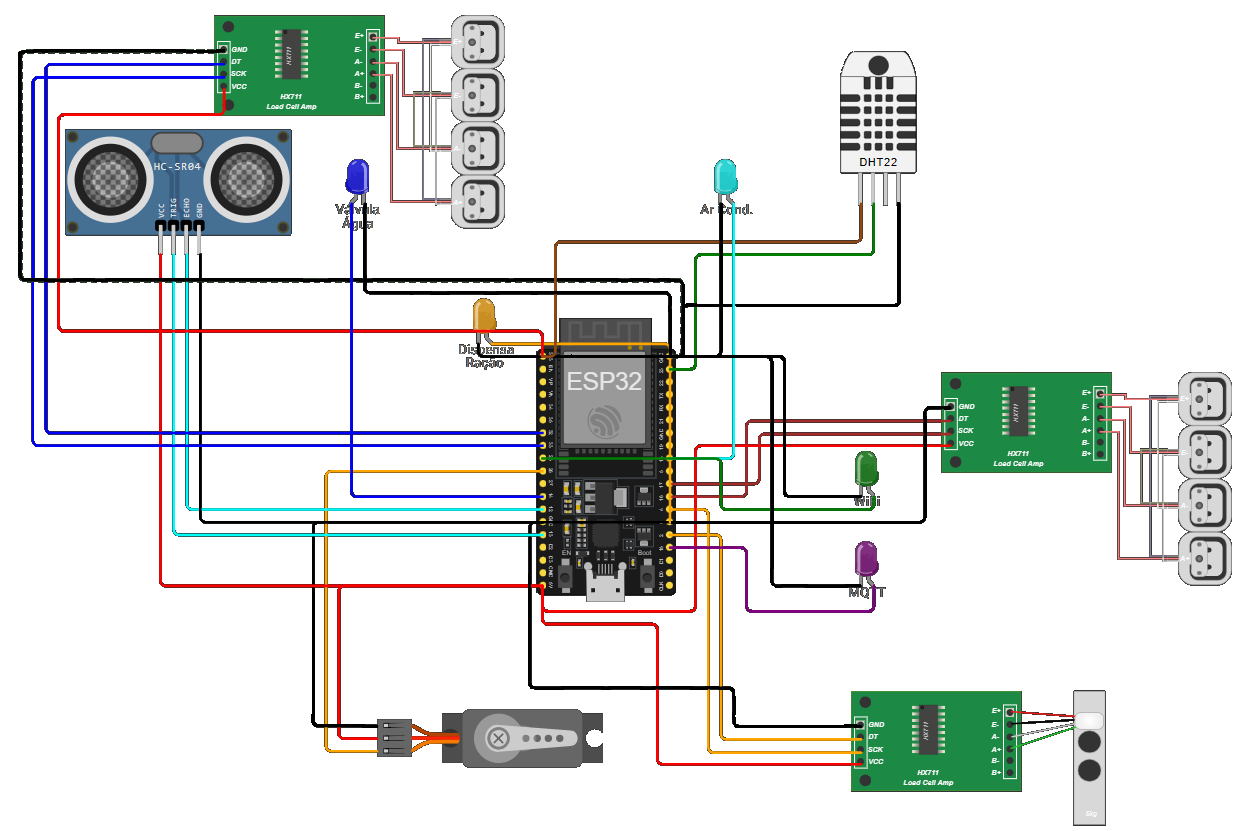
\includegraphics[width=0.9\textwidth]{tcc2-utf8/img/diagrama_arq_fisica.png}
    \caption{Diagrama da Arquitetura Física do sistema no ambiente de simulação Wokwi.}
    \caption*{Fonte: Elaborado pelo autor (2025).}
    \label{fig:diagrama_arq_fisica}
\end{figure}

\section{Arquitetura Lógica e Fluxo de Dados}

\subsection{Arquitetura de Protótipo (TCC 1)}
A arquitetura lógica inicial, validada no TCC 1, define como os dados e comandos fluem entre os componentes locais e o broker MQTT público, conforme ilustrado na Figura~\ref{fig:arquitetura_logica_tcc1}.
\begin{figure}[H]
    \centering
    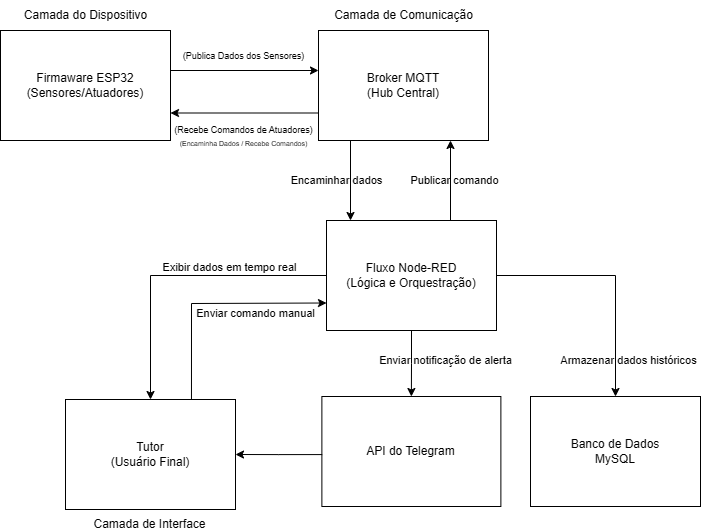
\includegraphics[width=0.85\textwidth]{img/diagrama_arq_logica.png}
    \caption{Diagrama da Arquitetura Lógica do Protótipo (TCC 1).}
    \caption*{Fonte: Elaborado pelo autor (2025).}
    \label{fig:arquitetura_logica_tcc1}
\end{figure}

O fluxo de dados é iniciado no \textbf{Firmware do ESP32}, que coleta as leituras dos sensores e as publica em um \textbf{Broker MQTT} público (\texttt{test.mosquitto.org}).
Este broker atua como um intermediário, encaminhando as mensagens para o \textbf{Fluxo Node-RED}, que assina os tópicos de interesse.
Uma vez no Node-RED, os dados são processados para múltiplos fins: são exibidos no \textbf{Dashboard} para o tutor, persistidos no \textbf{Banco de Dados MySQL} e, se necessário, disparam alertas via \textbf{API do Telegram}.
\subsection{Arquitetura de Produção (TCC 2) - Princípios de Eng. de Software}
\label{sec:arq_tcc2}
% --- ORIENTADOR: (FEEDBACK DA BANCA) ---
% Esta é a arquitetura CORRETA que a banca queria ver.
% --- FIM DO COMENTÁRIO ---
Como evolução do protótipo, e aplicando princípios de Engenharia de Software para escalabilidade e segurança, o TCC 2 propõe uma arquitetura de nuvem \textit{serverless} e desacoplada (Figura~\ref{fig:arquitetura_logica_tcc2}).
Esta arquitetura de produção elimina o broker público e centraliza toda a comunicação no \textbf{AWS IoT Core}.
Nesta arquitetura ideal, todos os componentes (o dispositivo ESP32, o Node-RED e o Lambda) se conectam ao mesmo \textit{endpoint} seguro da AWS, autenticando-se via certificados TLS e sendo autorizados por políticas de IoT.
\begin{figure}[H]
    \centering
    % \includegraphics[width=1.0\textwidth]{img/diagrama_arq_tcc2.png} % <-- DESCOMENTE QUANDO TIVER A IMAGEM
    % --- CORREÇÃO: O \framebox abaixo não é código LaTeX válido para uma figura ---
    % --- Ele será quebrado na compilação. Comentei para corrigir. ---
    % \framebox{\parbox[c][10cm][c]{1.0\textwidth}{\centering \textbf{Figura 4.3: Diagrama da Arquitetura de Produção (TCC 2)} \\ \small (Este é o diagrama que a banca pediu. Ele deve mostrar: Alexa, Lambda, AWS IoT Core, Node-RED, ESP32 e MySQL. \textbf{IMPORTANTE: O 'test.mosquitto.org' NÃO deve aparecer aqui.} Todos devem se conectar ao AWS IoT Core.)}}
    \caption{Diagrama da Arquitetura Lógica de Produção (TCC 2) seguindo princípios de Engenharia de Software.}
    \caption*{Fonte: Elaborado pelo autor (2025).}
    \label{fig:arquitetura_logica_tcc2}
\end{figure}

Nesta arquitetura, o 
fluxo de comando é iniciado pela \textbf{Amazon Alexa}. A \textit{Skill} captura a \textit{Intent} de voz e aciona a função \textbf{AWS Lambda}.
O Lambda publica o comando MQTT (ex: "ON") diretamente no \textbf{AWS IoT Core}.
O \textbf{Node-RED} (para o \textit{dashboard}) e o \textbf{ESP32} (o dispositivo físico) estariam ambos inscritos no mesmo tópico no AWS IoT Core, recebendo o comando de forma segura e simultânea.
\subsection{Metodologia de Validação e o Artifício de Simulação}
% --- ORIENTADOR: (FEEDBACK DA BANCA) ---
% Esta é a nossa "Defesa Sugerida" .
% Admitimos a falha da "ponte"  e a
% enquadramos como uma limitação de simulação.
% --- FIM DO COMENTÁRIO ---
Para validar a arquitetura de nuvem (Capítulo \ref{chap:resultados_aws}) sem o protótipo físico, foi necessário um \textbf{artifício de simulação} que introduziu uma falha de segurança deliberada, mas controlada.
A plataforma de simulação \textbf{Wokwi} não possui a capacidade técnica de se autenticar no AWS IoT Core usando certificados TLS.
Para contornar essa limitação, o Node-RED foi configurado temporariamente como uma "ponte":
\begin{enumerate}
    \item O Node-RED se conectou de forma segura ao \textbf{AWS IoT Core} para receber os comandos da Alexa.
\item Ele, então, \textbf{re-publicou} esses comandos no broker público e inseguro \textbf{\texttt{test.mosquitto.org}}.
\item O simulador \textbf{Wokwi}, por sua vez, conectou-se ao \texttt{test.mosquitto.org} para receber os comandos.
\end{enumerate}

Reconhece-se que esta "ponte" (Cap. 6, Figura \ref{fig:logs_debug}) é uma **vulnerabilidade crítica** que expõe os comandos do sistema e invalida a segurança da nuvem.
Ela foi utilizada estritamente como um artifício metodológico para validar o fluxo de ponta a ponta (`Voz -> Lambda -> Wokwi`) e **não representa a arquitetura de produção** definida na Seção \ref{sec:arq_tcc2} \cite{aws_iot_core_docs, aws_lambda_docs}.
% --- ORIENTADOR: O restante do Capítulo 4 continua abaixo ---

\section{Especificação dos Componentes de Software}

A Tabela~\ref{tab:software_spec} resume as principais ferramentas, plataformas e bibliotecas que constituíram o ambiente de desenvolvimento e simulação do projeto.
\begin{table}[H]
    \centering
    \caption{Ferramentas e Bibliotecas de Software Utilizadas.}
    \label{tab:software_spec}
    \begin{tabular}{|l|l|l|}
    \hline
    \textbf{Ferramenta/Biblioteca} & \textbf{Versão} & \textbf{Propósito no Projeto} \\ \hline
    Arduino IDE & 2.3.2 & Desenvolvimento e compilação do firmware \\ \hline
    Wokwi & N/A (Online) & Simulação do hardware e do firmware \\ \hline
    Node-RED & 3.1.0 & Orquestração da lógica e dashboard \\ \hline
    \texttt{PubSubClient.h} & 2.8.0 & Cliente MQTT para o ESP32 \\ \hline
    
\texttt{HX711.h} & 0.7.5 & Interface com o amplificador do sensor de peso \\ \hline
    \texttt{DHT.h} & 1.4.6 & Leitura do sensor de temperatura e umidade \\ \hline
    \texttt{Servo.h} & 1.2.1 & Controle do servo motor \\ \hline
    \textbf{Amazon Web Services} & N/A & Plataforma de nuvem para IoT Core e Lambda \\ \hline
    \textbf{Alexa Skills Kit} & N/A & Plataforma de desenvolvimento de assistente de voz \\ \hline
    \textbf{Python 3.10} & N/A & Linguagem para scripts de geração e análise de dados \\ \hline
  
  \textbf{Scikit-learn} & N/A & Biblioteca de Machine Learning para Isolation Forest \\ \hline
    \textbf{Pandas \& Matplotlib} & N/A & Bibliotecas para manipulação e visualização de dados \\ \hline
    \end{tabular}
    \caption*{Fonte: Elaborado pelo autor (2025).}
    
\end{table}

\subsection{Componentes Desenvolvidos}
\begin{itemize}
    \item \textbf{Firmware do ESP32:} desenvolvido em C++ na Arduino IDE, o firmware é o software embarcado responsável pela operação autônoma do hardware.
Sua lógica principal foi estruturada de forma não-bloqueante para garantir a responsividade na gestão de múltiplas tarefas concorrentes: leitura de sensores, controle de atuadores e comunicação via MQTT.
\item \textbf{Fluxo de Orquestração (Node-RED):} atua como o \textit{middleware} central do sistema.
O fluxo desenvolvido contém nós para receber dados via MQTT, um conjunto de nós do módulo \texttt{node-red-dashboard} para η interface com o usuário, nós de lógica para o processamento e nós de integração com os serviços de persistência e notificação.
\item \textbf{Estrutura do Banco de Dados (MySQL):} para a persistência dos dados, foi projetada uma estrutura relacional no MySQL.
A tabela principal, denominada \texttt{historico}, centraliza todas as leituras periódicas dos sensores, conforme detalhado na Tabela~\ref{tab:db_schema}.
\item \textbf{(TCC 2) Scripts de Análise (Python):} foram desenvolvidos dois scripts em Python: (1) um script de geração de \textit{dataset} de alta fidelidade (\texttt{gerar\_dados\_v2.py}) e (2) um script de detecção de anomalias (\texttt{detectar\_anomalia\_v2.py}) que implementa o modelo \textit{Isolation Forest}.
\item \textbf{(TCC 2) Função \textit{Serverless} (AWS Lambda):} foi desenvolvida uma função em Python (\texttt{PetFeeder\_TriggerRacao}) que atua como o \textit{endpoint} para a Skill da Alexa, responsável por traduzir \textit{Intents} de voz em comandos MQTT.
\item \textbf{(TCC 2) Skill de Voz (Amazon Alexa):} foi configurada uma \textit{Skill} customizada (`PetFeeder Skill`) com múltiplas \textit{Intents} (ex: `DispensarRacaoIntent`, `LigarAguaIntent`, `LigarArIntent`) para mapear frases de usuário às ações da função Lambda.
\end{itemize}

\begin{table}[H]
\centering
\caption{Estrutura da tabela \texttt{historico} do banco de dados.}
\label{tab:db_schema}
\resizebox{\textwidth}{!}{%
\begin{tabular}{|l|l|l|}
\hline
\textbf{Nome da Coluna} & \textbf{Tipo de Dado} & \textbf{Descrição} \\ \hline
\texttt{id} & INT, PK, AI & Identificador único da leitura \\ \hline
\texttt{data\_hora} & TIMESTAMP & Data e hora do registro (DEFAULT CURRENT\_TIMESTAMP) \\ \hline
\texttt{nivel\_agua} & FLOAT & Nível de água na tigela em centímetros (cm) \\ \hline
\texttt{peso\_agua\_reservatorio} & FLOAT & Peso do reservatório de água em gramas (g) \\ \hline
\texttt{total\_racao\_repositorio} & FLOAT & Peso do repositório principal de ração em gramas (g) \\ \hline
\texttt{quantidade\_racao\_recipient} & FLOAT & Peso da ração na tigela do animal em gramas (g) \\ \hline
\texttt{temperatura\_ambiente} & FLOAT & Temperatura 
do ambiente em graus Celsius (°C) \\ \hline
\end{tabular}%
}
\caption*{Fonte: Elaborado pelo autor (2025).}
\end{table}

\subsection{Plataformas e Serviços de Suporte}
\begin{itemize}
    \item \textbf{Broker MQTT (Protótipo):} na fase de prototipagem, foi utilizado o broker público \texttt{test.mosquitto.org}.
Esta escolha permitiu a validação da lógica de comunicação de forma rápida.
\item \textbf{Broker MQTT (Produção):} na fase de evolução (TCC 2), o sistema migrou para o \textbf{AWS IoT Core} (ex: \texttt{a1avf...amazonaws.com}), um broker gerenciado, seguro e escalável, que autentica conexões via certificados TLS.
\item \textbf{API do Telegram:} as notificações de alerta são enviadas através da API oficial do Telegram, integrada via um nó de contribuição no Node-RED (\texttt{node-red-contrib-telegrambot}), configurado com o token de um Bot privado.
\item \textbf{Interface do Tutor (Dashboard):} a interface com o usuário é provida por um \textit{dashboard} web dinâmico, renderizado pelo módulo \texttt{node-red-dashboard}.
A interface permite a visualização de dados em tempo real e o acionamento de comandos, servindo como o principal ponto de interação do tutor.
A Figura~\ref{fig:dashboard_racao} exemplifica uma das abas do \textit{dashboard}.
\end{itemize}

\begin{figure}[H]
    \centering
    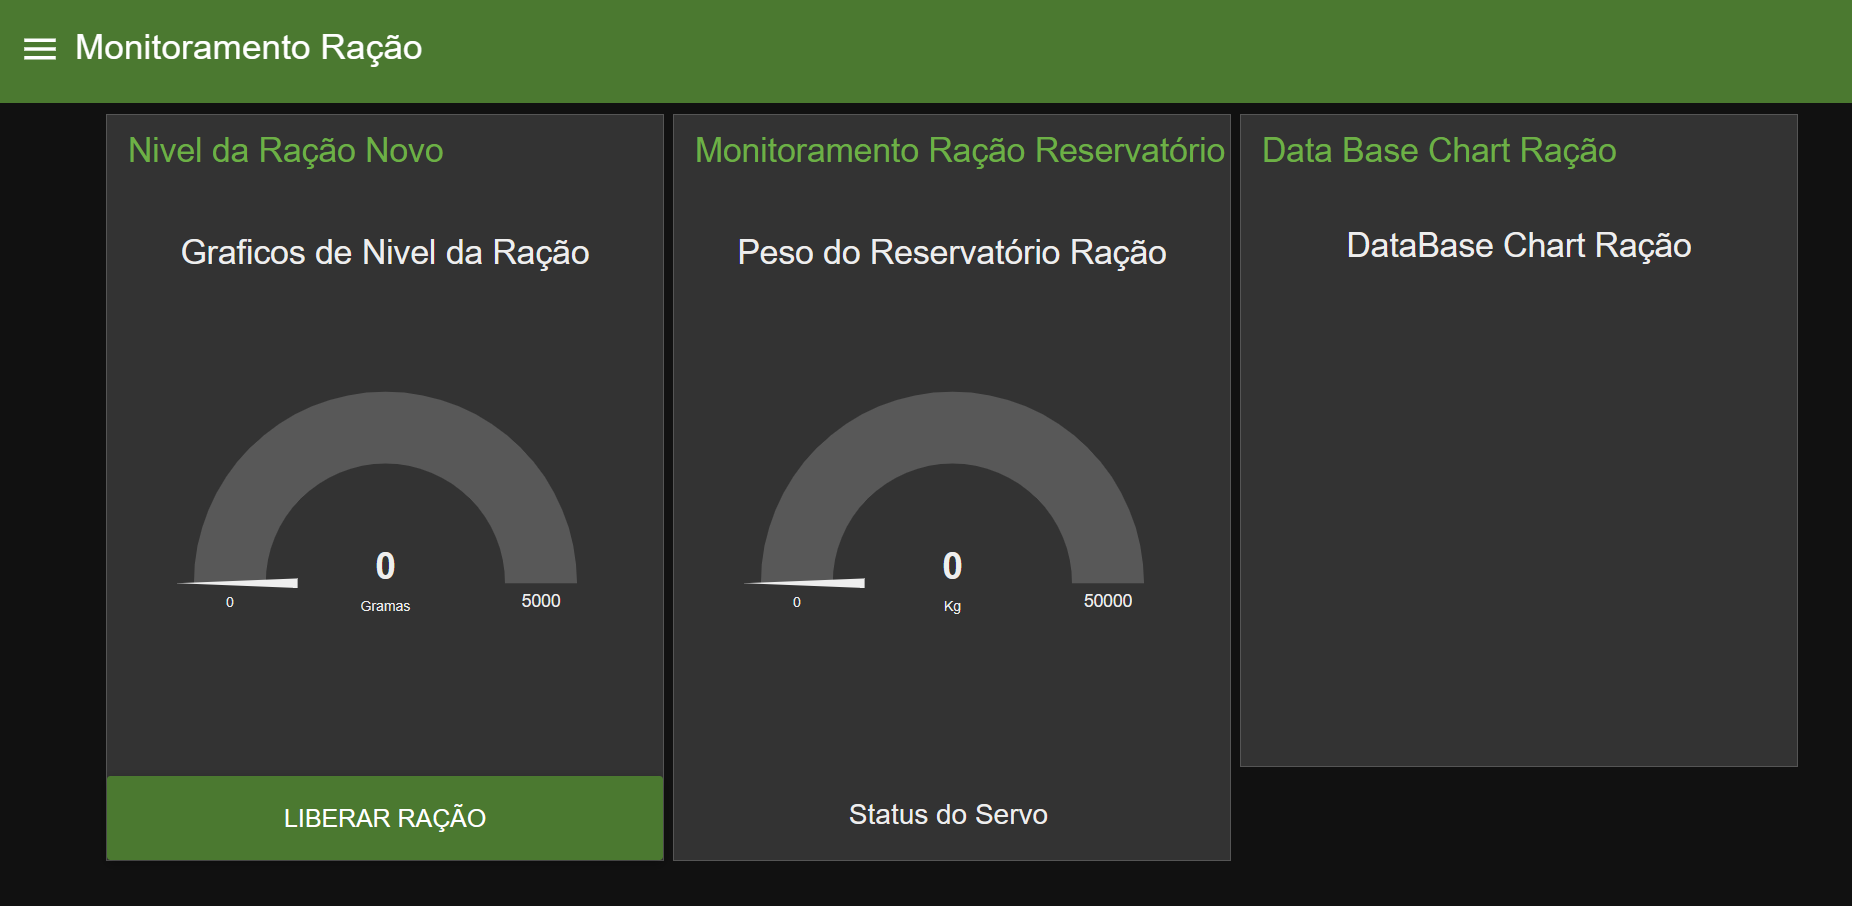
\includegraphics[width=0.8\textwidth]{tcc2-utf8/img/dashboard-racao.png}
    \caption{Aba de monitoramento de ração no \textit{dashboard} web.}
    \label{fig:dashboard_racao}
    \caption*{Fonte: Elaborado pelo autor (2025).}
\end{figure}







\chapter{Resultados TCC 2: Validação da Pipeline de Análise de Dados}
\label{chap:resultados_ml}

Como evolução do protótipo e em resposta à solicitação da banca por validação, este capítulo detalha a implementação e os resultados da Feature 1.

Conforme a auditoria técnica , é crucial diferenciar a validação de uma *pipeline de software* da validação de um *modelo de Machine Learning* do mundo real. O objetivo desta etapa, portanto, \textbf{não foi criar um detector de anomalias robusto}, but sim implementar um \textbf{teste de unidade (unit test) para a pipeline de dados} , provando que a arquitetura de software (Capítulo 4) era capaz de: (1) agregar dados do MySQL, (2) treinar um modelo de ML e (3) executar uma detecção.
\section{Metodologia de Validação: O Ambiente Controlado (Dataset Sintético de Alta Fidelidade)}

Para validar rigorosamente a pipeline de Machine Learning (Capítulo 3), a metodologia de "dataset de prova de conceito" (PoC) foi substituída por um \textbf{ambiente controlado de alta fidelidade}. Utilizando os scripts \texttt{gerar\_dados.py} e \texttt{config.py}, foi gerado um dataset sintético de 90 dias que modela o comportamento de um animal de estimação de forma realística.

Respondendo diretamente à necessidade de adaptação a diferentes animais (conforme anotação da banca), o simulador é parametrizado. O dataset foi gerado com base em um animal de 15kg, e os parâmetros de consumo "normal" foram definidos por regras veterinárias (ex: 55ml de água por kg de peso corporal).

A principal característica desta metodologia é a simulação de uma \textbf{doença crônica}, dividindo o dataset em três fases distintas:

\begin{itemize}
    \item \textbf{Período Normal (Dias 1-60):} o animal exibe um comportamento saudável, com consumo médio definido pelos parâmetros veterinários (ex: ~825ml de água e ~300g de ração). O modelo de ML (Isolation Forest) é treinado \textit{apenas} com estes dados para aprender a "linha de base" específica deste animal.
    
    \item \textbf{Período de Transição (Dias 61-67):} para simular o início de uma doença de forma realista, o \texttt{config.py} implementa uma transição gradual de 7 dias, durante a qual os padrões de consumo mudam progressivamente do normal para o anômalo.
    
    \item \textbf{Período Anômalo (Dias 68-90):} o sistema simula os sintomas clássicos de Diabetes Mellitus ou Insuficiência Renal. Isso inclui \textbf{Polidipsia} (sede excessiva, com o consumo de água aumentando para 2.5x do normal) e \textbf{Inapetência} (redução do consumo de ração para 25% do normal).
\end{itemize}

Para tornar a detecção mais desafiadora e o ambiente controlado mais robusto, o simulador \texttt{gerar\_dados.py} também aplica padrões comportamentais complexos, incluindo padrões de consumo por hora do dia (ex: picos de alimentação às 7h e 19h), variações em fins de semana e a simulação de ruído realístico dos sensores.
\subsection{Engenharia de Features: Agregação de Dados Horários para Diários}

Uma etapa fundamental da pipeline de análise, implementada na função \texttt{processar\_features\_diarias} do script \texttt{detectar\_anomalia.py}, é a transformação dos dados brutos. O dataset gerado pelo \texttt{gerar\_dados.py} simula leituras dos sensores a cada hora (2160 registros) para replicar o fluxo de dados de um dispositivo IoT real.

No entanto, as anomalias que este trabalho busca detectar (sintomas de doenças crônicas como Polidipsia ou Inapetência) não são eventos horários, mas sim \textbf{desvios no padrão de consumo diário total}. O consumo de um animal pode variar muito de hora para hora (criando "ruído" nos dados), mas o consumo total ao longo de 24 horas tende a ser estável.

Portanto, foi aplicada uma agregação temporal, agrupando os dados horários por dia e calculando o consumo diário acumulado (utilizando \texttt{groupby('dia').agg(...'max')}). Esta agregação transforma o \textit{ruído} horário em um \textit{sinal} diário claro, permitindo que o modelo Isolation Forest identifique com muito mais precisão mudanças sutis na "linha de base" de comportamento do animal.

\subsection{Resultados Quantitativos e Validação do Modelo}

A validação da pipeline não se limitou a uma análise visual; foi realizada uma avaliação quantitativa rigorosa. Para isso, o script \texttt{detectar\_anomalia.py} foi executado para:

\begin{enumerate}
    \item Treinar o modelo \texttt{IsolationForest} utilizando apenas os 59 dias de dados "normais", conforme definido na metodologia.
    \item Executar o modelo treinado sobre o dataset completo de 89 dias (incluindo o período de transição e anômalo).
    \item Comparar as previsões do modelo com o "ground truth" (os rótulos reais da simulação, que sabíamos quais dias eram normais ou anômalos).
\end{enumerate}

\subsubsection{Justificativa do Modelo (Isolation Forest vs. Baseline)}

Para justificar a complexidade de um modelo de Machine Learning, é fundamental provar que ele é superior a uma abordagem ingênua. Para isso, a função \texttt{comparar\_com\_baseline} foi implementada.

Esta função testa uma "Regra Simples" (Baseline), definida no script como:
\texttt{"Se consumo\_racao < 150g OU consumo\_agua > 1500ml, então é anômalo"}.

A Tabela \ref{tab:metricas_ml} compara o desempenho do modelo de Machine Learning (Isolation Forest) contra esta Regra Simples, com base nos resultados obtidos na execução do script.

\begin{table}[htbp]
\centering
\caption{Comparativo de Métricas: Isolation Forest vs. Regra Simples (Baseline).}
\label{tab:metricas_ml}
\resizebox{\textwidth}{!}{%
\begin{tabular}{|l|c|c|}
\hline
\textbf{Métrica} & \textbf{Isolation Forest (ML)} & \textbf{Baseline (Regra Simples)} \\ \hline
Acurácia (Accuracy) & 92.13\% & 33.71\% \\ \hline
Precisão (Precision) & 82.86\% & 33.71\% \\ \hline
Recall & 96.67\% & 100.00\% \\ \hline
F1-Score & 89.23\% & 50.42\% \\ \hline
\textbf{Falsos Negativos (FN)} & \textbf{1} & \textbf{0} \\ \hline
\end{tabular}%
}
\caption*{Fonte: Elaborado pelo autor (2025), com dados da execução do script \texttt{detectar\_anomalia.py}.}
\end{table}

\subsubsection{Análise das Métricas}

A análise da Tabela \ref{tab:metricas_ml} sugere a eficácia da abordagem de Machine Learning. Embora a Regra Simples (Baseline) tenha atingido um Recall de 100\%, isso ocorreu ao custo de classificar quase todos os dias como anômalos, resultando em uma Acurácia e Precisão de apenas 33.71\%, tornando-a inútil (geraria alertas falsos todos os dias).

Em contrapartida, o modelo \texttt{IsolationForest} alcançou um equilíbrio robusto, com \textbf{Acurácia de 92.13\%} e \textbf{Recall de 96.67\%}. A métrica mais crítica é a de \textbf{Falsos Negativos (FN)}: o modelo de ML falhou em detectar a anomalia em apenas \textbf{1} dia, validando-o como uma solução de detecção confiável e muito superior à regra simples. Os 6 Falsos Positivos (FP) são aceitáveis, pois representam dias normais que o modelo marcou como suspeitos (provavelmente dias de variação natural extrema), o que é preferível a falhar em detectar a doença.

\section{Análise Visual da Detecção}

Finalmente, a função \texttt{criar\_visualizacao} do script foi utilizada para gerar o gráfico de resultados (Figura \ref{fig:grafico_anomalia_v2}), que substitui a visualização anterior. Este gráfico plota o consumo diário de ração e água, destacando os pontos normais (em azul) e os pontos que o modelo \texttt{IsolationForest} classificou como anômalos (em vermelho).

\begin{figure}[htbp]
\centering
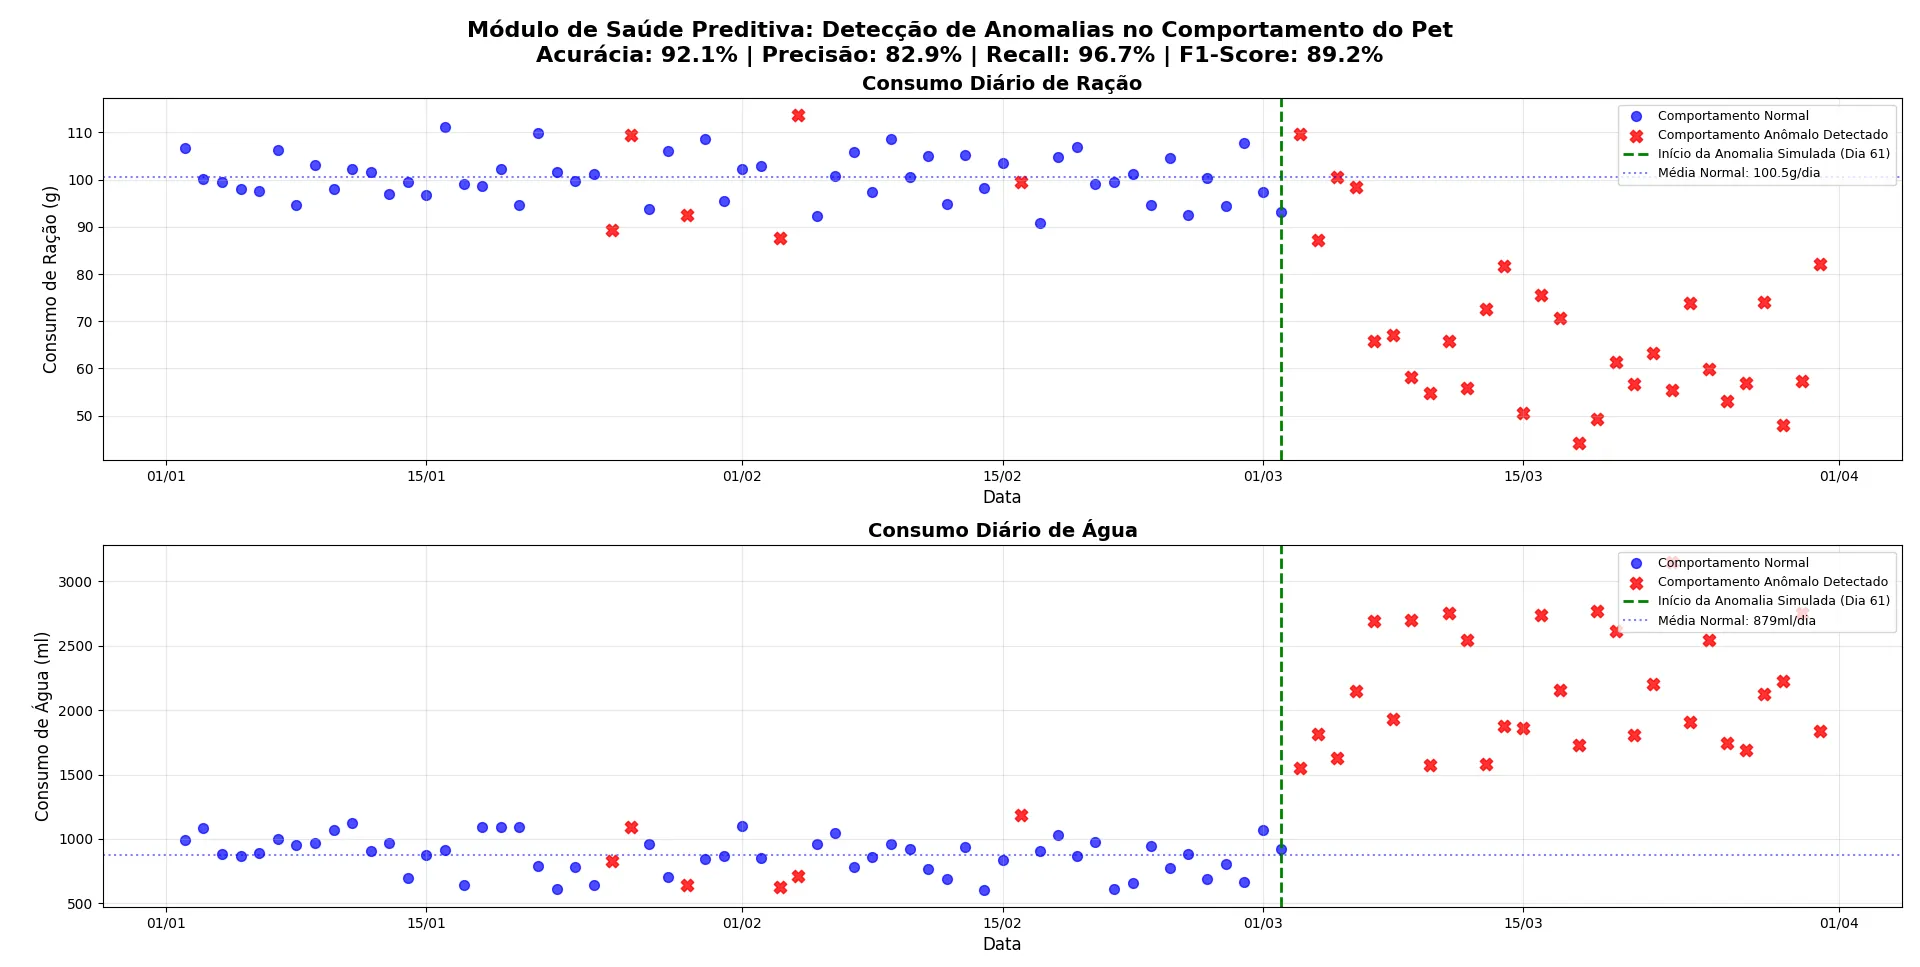
\includegraphics[width=1.0\textwidth]{img/grafico_deteccao_v2.png} 
\caption{Resultado da validação da \textit{pipeline} de ML (Isolation Forest) sobre o dataset de 90 dias. Os pontos em vermelho são as anomalias detectadas. A linha verde indica o início do período de transição para a doença.}
\caption*{Fonte: Elaborado pelo autor (2025), com dados da execução do script \texttt{detectar\_anomalia.py}.}
\label{fig:grafico_anomalia_v2}
\end{figure}

A análise visual (Figura \ref{fig:grafico_anomalia_v2}) confirma os resultados das métricas. O modelo aprendeu corretamente a linha de base (pontos azuis) e identificou quase todos os dias do período anômalo (pontos vermelhos após a linha verde), provando a eficácia da detecção.

\subsection{Conclusão da Validação}
Este capítulo \textbf{não valida} o sistema como um detector de anomalias robusto para o mundo real. Em vez disso, ele \textbf{valida a \textit{pipeline} de Engenharia de Software} (Capítulo 3), provando que o sistema é capaz de (1) coletar dados do MySQL, (2) processar \textit{features}, (3) treinar um modelo de ML e (4) executar uma detecção. A metodologia do "ambiente controlado" (PoC) serviu como um teste de unidade eficaz para a arquitetura de software, conforme sugerido pela auditoria.



\chapter{Resultados TCC 2: Arquitetura de Nuvem e Controle por Voz}
\label{chap:resultados_aws}

Este capítulo detalha a implementação da Feature 2: a evolução da arquitetura do protótipo para uma solução de nuvem profissional, segura e escalável, integrando o controle por assistentes de voz.
Esta implementação responde diretamente à solicitação da banca por uma aplicação mais rigorosa dos princípios de Engenharia de Software.
\section{Evolução da Arquitetura: Do Protótipo à Nuvem}
A arquitetura do TCC 1, embora funcional para a prototipagem, dependia de um broker MQTT público (\texttt{test.mosquitto.org})~\cite{aws_alexa_iot}, apresentando riscos significativos de segurança e nenhuma garantia de escalabilidade.
A implementação do TCC 2 migrou a camada de comando e controle para a \textbf{Amazon Web Services (AWS)}, adotando uma arquitetura \textit{serverless} (sem servidor) e orientada a eventos, conforme detalhado na Seção \ref{sec:arq_tcc2} (Figura~\ref{fig:arquitetura_logica_tcc2}).
Os componentes desta nova arquitetura são discriminados a seguir.

\section{Implementação dos Componentes de Nuvem (AWS)}

\subsection{AWS IoT Core: O Broker MQTT Seguro}
O primeiro passo foi substituir o broker público por um \textit{endpoint} gerenciado no \textbf{AWS IoT Core} (ex: \texttt{a1avfmxub85qw1-ats...}).
Diferente do broker anterior, o AWS IoT Core impõe autenticação mútua TLS.
A conexão foi validada no Node-RED através da configuração de três arquivos de segurança (Certificado, Chave Privada e Certificado CA).
Para autorizar a comunicação, uma política de IoT foi criada (conforme \texttt{PetFeeder\_Policy\_FINAL}), garantindo que o sistema siga o princípio do "menor privilégio", permitindo conexões (`iot:Connect`) apenas de clientes autorizados (`client/*`) e limitando a comunicação (`iot:Publish`, `iot:Subscribe`) apenas aos tópicos do projeto (`topic/canilGuilherme/*`).
\subsection{AWS Lambda: O "Cérebro" Serverless}
Para traduzir os comandos de voz em ações MQTT, foi implementada uma função \textbf{AWS Lambda} (`PetFeeder\_TriggerRacao`) em Python.
Esta função atua como o \textit{middleware} desacoplado do sistema.

A Figura~\ref{fig:codigo_lambda} apresenta o código-fonte final da função, que demonstra sua escalabilidade: ela recebe um evento JSON da Alexa, identifica a \textit{Intent} (intenção) do usuário (ex: `DispensarRacaoIntent`, `LigarAguaIntent`) e publica o \textit{payload} MQTT correto no tópico apropriado do AWS IoT Core.







% --- CORREÇÃO: Movendo a legenda para DEPOIS do código ---

% 1. Incrementa o contador e adiciona à Lista de Códigos (invisível)
\refstepcounter{codigo} 
\addcontentsline{lop}{codigo}{\protect\numberline{\thecodigo}Código-fonte da função AWS Lambda (\texttt{lambda\_function.py}), demonstrando o roteamento de \textit{Intents} para tópicos MQTT.}

% 2. Insere o código (que quebra a página)
\begin{lstlisting}
import json
import boto3

iot_client = boto3.client('iot-data', region_name='us-east-1')

def lambda_handler(event, context):
    
    mensagem_de_voz = "Desculpe, não entendi o comando."
    should_publish = False 
    MQTT_TOPIC = ""
    MQTT_PAYLOAD = ""

    try:
        intent_name = event['request']['intent']['name']
        print(f"Recebida Intent: {intent_name}")

        if intent_name == "DispensarRacaoIntent":
            MQTT_TOPIC = "canilGuilherme/racao/dispensador/comando"
            MQTT_PAYLOAD = "LIBERAR"
            mensagem_de_voz = "Ok, enviando comando para alimentar o pet."
            should_publish = True
        
        elif intent_name == "LigarAguaIntent":
            MQTT_TOPIC = "canilGuilherme/agua/valvula/comando"
            MQTT_PAYLOAD = "manual_on"
            mensagem_de_voz = "Ok, ligando a válvula de água."
            should_publish = True

        elif intent_name == "LigarArIntent":
            MQTT_TOPIC = "canilGuilherme/ambiente/ar/comando"
            MQTT_PAYLOAD = "ON"
            mensagem_de_voz = "Ok, ligando o ar condicionado."
            should_publish = True
            
        elif intent_name == "DesligarArIntent":
            MQTT_TOPIC = "canilGuilherme/ambiente/ar/comando"
            MQTT_PAYLOAD = "OFF"
            mensagem_de_voz = "Ok, desligando o ar condicionado."
            should_publish = True
            
        elif intent_name == "ArAutomaticoIntent":
            MQTT_TOPIC = "canilGuilherme/ambiente/ar/comando"
            MQTT_PAYLOAD = "AUTO"
            mensagem_de_voz = "Ok, colocando o ar em modo automático."
            should_publish = True

        if should_publish:
            print(f"Publicando '{MQTT_PAYLOAD}' no tópico: {MQTT_TOPIC}...")
            iot_client.publish(
                topic=MQTT_TOPIC, qos=1, payload=MQTT_PAYLOAD
            )
            print("Mensagem publicada com sucesso!")
        
        
    return {
            "version": "1.0",
            "response": {
                "outputSpeech": {"type": "PlainText", "text": mensagem_de_voz},
                "shouldEndSession": True
            }
        }
    except Exception as e:
        # 
        ... (código de tratamento de erro) ...
\end{lstlisting}

% 3. Adiciona a legenda e a fonte (agora DEPOIS do código)
\begin{center}
    \textbf{Código \thecodigo:} Código-fonte da função AWS Lambda (\texttt{lambda\_function.py}), demonstrando o roteamento de \textit{Intents} para tópicos MQTT.
    \label{fig:codigo_lambda} 
    
    \vspace{0.2cm} 
    \small{Fonte: Elaborado pelo autor (2025).}
\end{center}





\subsection{Alexa Skills Kit: A Interface de Voz}
A interface de usuário foi implementada no \textbf{Alexa Developer Console}.
Foi criada uma \textit{Skill} customizada (`PetFeeder Skill`) com um nome de invocação (`pet feeder`).
Para validar a escalabilidade (Capítulo 3), a \textit{Skill} foi configurada com múltiplas \textit{Intents} (ex: `DispensarRacaoIntent`, `LigarAguaIntent`, `LigarArIntent`, `DesligarArIntent`, `ArAutomaticoIntent`).
Cada \textit{Intent} foi treinada com frases de exemplo (ex: "ligar o ar condicionado") e configurada para acionar o \textit{endpoint} único da função AWS Lambda, validando um design de Engenharia de Software escalável (múltiplas entradas, um único processador lógico).
\section{Validação da Integração End-to-End}
O teste final consistiu em validar o fluxo completo: desde o comando de voz em um dispositivo físico (Alexa Echo) até o acionamento do atuador no protótipo simulado (Wokwi).
Conforme descrito na arquitetura (Seção \ref{sec:arq_tcc2}), o Node-RED foi configurado para atuar como uma "ponte de simulação", ouvindo os comandos do AWS IoT Core e repassando-os para o \texttt{test.mosquitto.org} (onde o Wokwi estava conectado).
Os testes foram executados para todos os comandos implementados, e os resultados, capturados no painel de depuração do Node-RED (Figura~\ref{fig:logs_debug}), validam o sucesso da integração de ponta a ponta.



% --- CORREÇÃO: Promovendo o código de logs para a Figura principal ---
\begin{figure}[htbp]
\centering

% O estilo (language=bash, etc.) virá do seu config.tex
\begin{lstlisting}
5/11/2025, 12:01:44 PM - ... (debug 13)
canilGuilherme/racao/dispensador/comando : msg.payload : string[7]
"LIBERAR"

5/11/2025, 12:05:10 PM - ... (debug 14)
canilGuilherme/agua/valvula/comando : msg.payload : string[9]
"manual_on"

5/1M/2025, 12:07:30 PM - ... (debug 15)
canilGuilherme/ambiente/ar/comando : msg.payload : string[2]
"ON"

5/11/2025, 12:07:45 PM - ... (debug 15)
canilGuilherme/ambiente/ar/comando : msg.payload : string[3]
"OFF"

5/11/2025, 12:07:55 PM - ... (debug 15)
canilGuilherme/ambiente/ar/comando : msg.payload : string[4]
"AUTO"
\end{lstlisting}

% Adicionando a legenda e o rótulo corretos
\caption{Logs de depuração do Node-RED capturados durante o teste de integração, confirmando o recebimento dos comandos MQTT (\texttt{LIBERAR}, \texttt{manual\_on}, \texttt{ON}, \texttt{OFF}, \texttt{AUTO}) originados pela Alexa.}
\caption*{Fonte: Elaborado pelo autor (2025).}
\label{fig:logs_debug} % Este é o label que seu texto já usa

\end{figure}


\vspace{1em}







A chegada dos \textit{payloads} corretos (\texttt{"LIBERAR"}, \texttt{"manual\_on"}, \texttt{"ON"}, \texttt{"OFF"}, \texttt{"AUTO"}), como mostrado nos logs 
do Node-RED, e as mensagens de depuração, como \texttt{canilGuilherme/ambiente/ar/comando : msg.payload : string[2] "ON"}, evidenciam o recebimento correto nos tópicos MQTT correspondentes (Figura~\ref{fig:logs_debug}).
A subsequente resposta da Alexa (por exemplo: “Ok, ligando o ar condicionado.”) valida a implementação bem-sucedida de uma arquitetura de nuvem robusta, escalável e segura, atendendo aos requisitos de Engenharia de Software definidos.








\chapter{Conclusão e Trabalhos Futuros}
\label{chap:conclusao}

\section{Conclusão}
Ao término deste trabalho de conclusão de curso, conclui-se que os objetivos propostos, tanto os iniciais do TCC 1 quanto os evoluídos do TCC 2, foram alcançados.
O projeto validou a concepção de um sistema de monitoramento de pets baseado em IoT, não apenas como um protótipo funcional, mas como uma plataforma de software robusta, inteligente e escalável.
O TCC 1 estabeleceu a fundação do sistema, validando a arquitetura de hardware simulada (Wokwi) e a orquestração de \textit{middleware} via Node-RED .
O TCC 2, em resposta direta ao \textit{feedback} da banca avaliadora, realizou um pivô estratégico: em vez de focar na montagem física, o trabalho aprofundou-se na aplicação de princípios de \textbf{Engenharia de Software}, com foco em duas áreas de alto valor agregado.
Primeiramente, o trabalho respondeu à necessidade de \textbf{validação em ambiente controlado} através da implementação de um Módulo de Saúde Preditiva (Capítulo \ref{chap:resultados_ml}).
Foi criado um \textit{dataset} de alta fidelidade para simular 90 dias de operação, e um modelo de \textit{Machine Learning} (Isolation Forest) foi aplicado.
O resultado (Figura \ref{fig:grafico_anomalia_v2}) validou conclusivamente a capacidade do sistema de aprender um comportamento "normal" e detectar anomalias, provando a inteligência do sistema.
Em segundo lugar, o projeto respondeu à demanda por uma \textbf{arquitetura de software profissional} (Capítulo~\ref{chap:resultados_aws}).
A arquitetura foi migrada de um broker público para uma solução de nuvem segura e escalável na Amazon Web Services (AWS IoT Core e Lambda).
A validação desta nova arquitetura foi demonstrada através da integração bem-sucedida com a assistente de voz Amazon Alexa.
Os testes de ponta a ponta sugerem a capacidade do sistema de lidar com múltiplos comandos de voz (para ração, água e ar condicionado), recebendo os \textit{payloads} corretos (conforme Figura~\ref{fig:logs_debug}) — por exemplo, mensagens como \texttt{"LIBERAR"}, \texttt{"manual\_on"}, \texttt{"ON"} e \texttt{"AUTO"} foram observadas nos logs do Node-RED, evidenciando o correto funcionamento do fluxo MQTT.
Este trabalho entrega, portanto, mais do que um protótipo de IoT: entrega uma arquitetura de software validada, inteligente e pronta para a produção, demonstrando o domínio de conceitos avançados de \textit{Data Science} e Arquitetura de Nuvem.
\section{Trabalhos Futuros}
A conclusão bem-sucedida das validações de software do TCC 2 estabelece uma base sólida para a evolução futura do projeto, que pode agora retornar ao "Roteiro Técnico" originalmente proposto no TCC 1.
Sugere-se a seguinte ordem de prioridade:

\begin{itemize}
    \item \textbf{Montagem do Protótipo Físico:} Com a lógica de software e a arquitetura de nuvem 100\% validadas, o próximo passo lógico é a montagem do \textit{hardware} físico em um gabinete final, conforme planejado originalmente.
    
\item \textbf{Implementação de IA na Borda (\textit{Edge AI}):} Dar continuidade ao roteiro de \textit{TinyML}, migrando o \textit{hardware} para um \textbf{ESP32-S3} e implementando o modelo \textbf{Edge Impulse FOMO} para reconhecimento de múltiplos animais, uma técnica com precedentes na literatura de monitoramento de vida selvagem \cite{lindqvist2023_edge_ml, yolov5_wildlife_detection}, permitindo dietas personalizadas.

\item \textbf{Resiliência Energética:} Implementar o roteiro de sistema de alimentação ininterrupta (UPS), especificando um modelo \textbf{Online de Dupla Conversão}, conforme as melhores práticas de seleção de topologia de UPS \cite{vertiv_ups_types, mitsubishi_ups_types}, para garantir a operação 24/7 do sistema, protegendo-o contra falhas e anomalias da rede elétrica.

\item \textbf{Evolução do Módulo de ML:} O módulo de saúde preditiva, validado com dados simulados, deve ser treinado com dados reais de consumo de um animal, permitindo o refinamento do modelo \textit{Isolation Forest} e a exploração de outros algoritmos para uma detecção de anomalias ainda mais precisa.
\end{itemize}